\documentclass[11pt]{article}
\usepackage{vntex}
\usepackage[english]{babel}
\usepackage[utf8]{inputenc}
\usepackage[colorlinks = true,
            linkcolor = blue,
            urlcolor  = blue]{hyperref}
\usepackage[a4paper,margin=1.5in]{geometry}
\usepackage{stackengine,graphicx}
\usepackage{fancyhdr}
\setlength{\headheight}{15pt}
\usepackage{microtype}
\usepackage{times}
\usepackage{booktabs}
\usepackage{gensymb}
\usepackage{amsmath}
\usepackage{float}

% python code format: https://github.com/olivierverdier/python-latex-highlighting
\usepackage{pythonhighlight}

\frenchspacing
\setlength{\parindent}{0cm} % Default is 15pt.
\setlength{\parskip}{0.3cm plus1mm minus1mm}

\pagestyle{fancy}
\fancyhf{}
\lhead{Local Feature Matching}
\rhead{Xử lý ảnh số và thị giác máy tính}
\rfoot{\thepage}

\date{}

\title{\vspace{-1cm}Bài tập lớn 2: Local Feature Matching}

\begin{document}
\maketitle
\vspace{-2cm}
\thispagestyle{fancy}

\section*{Giới thiệu}
Bài tập lớn này tập trung vào việc so trùng đặc trưng giữa hai ảnh. Bao gồm ba bước chính:
\begin{itemize}
    \item Interest detection point: Xác định các vị trí key points trong ảnh bằng cách hiện thực giải thuật Harris Corner Detector.
    \item Local feature description: Biểu diễn các đặc trưng, các vùng xung quanh vị trị trong ảnh dưới dạng một vector gọi là vector đặc trưng bằng cách hiện thực giải thuật Scale-Invarient feature transform (SIFT).
    \item Feature matching: So trùng các đặc trưng bằng cách tính toán khoảng cách giữa các điểm đặc trưng và tìm ra các điểm tương đồng bằng cách hiện thực giải thuật Nearest Neighbor Distance Ratio.
\end{itemize}

\section*{Chi tiết hiện thực}
\subsection*{Interest detection point}
Tìm ra tập các điểm được xem là quan trọng. Các bước hiện thực giải thuật Harris Corner Detector:
\begin{enumerate}
    \item Blur ảnh trước để tránh nhiễu trong ảnh bằng cách sử dụng gaussian filter.
    \item Tính toán đạo hàm của ảnh theo hai trục x trục y bằng sobel filter theo 2 trục.
        \begin{equation*}
            \nabla I_0(x_i) = (\frac{\partial I_0}{\partial x}, \frac{\partial I_0}{\partial y})(x_i)
        \end{equation*}
    \item Tính toán các tham số $g(I_x^2), g(I_y^2), g(I_{xy})$ trong đó g là gaussian filter.
    \item Trên mỗi điểm ảnh:
        \begin{itemize}
            \item Tính các tham số sau:
                \begin{equation*}
                    S_{xx} = \sum_{x, y} g(I_x^2)
                \end{equation*}
                \begin{equation*}
                    S_{yy} = \sum_{x, y} g(I_y^2)
                \end{equation*}
                \begin{equation*}
                    S_{xy} = \sum_{x, y} g(I_{xy})
                \end{equation*}
            \item Tính độ đo C bằng công thức sau:
                \begin{equation*}
                    C = S_{xx} \circ S_{yy} - S_{xy}^2 - alpha*(S_{xx} + S_{yy})^2
                \end{equation*}
            \item Chọn các điểm key points dựa vào ngưỡng threshold:
        \end{itemize}
    \item Áp dụng non-non-maximal suppression để loại bỏ các điểm có khoảng cách dưới min-distance.
\end{enumerate}
Chi tiết hiện thực giải thuật Harris Corner Detector trên python:
\inputpython{code/get_interest_points.py}{1}{43}

\subsection*{Local feature description}
Mô tả các điểm bằng một vector đặc trưng 128 chiều. Các bước hiện thực giải thuật Scale-Invarient feature transform (SIFT):
\begin{enumerate}
    \item Blur ảnh trước để tránh nhiễu trong ảnh bằng cách sử dụng gaussian filter.
    \item Tính toán đạo hàm của ảnh theo hai trục x trục y bằng sobel filter theo 2 trục.
        \begin{equation*}
            \nabla I_0(x_i) = (\frac{\partial I_0}{\partial x}, \frac{\partial I_0}{\partial y})(x_i)
        \end{equation*}
    \item Tính độ lớn và góc của gradient dựa theo đạo hàm của ảnh theo hai trục.
        \begin{equation*}
            magnitude\_gradient = \sqrt{I_x^2 + I_y^2}
        \end{equation*}
        \begin{equation*}
            direction\_gradient = \arctan{(I_x, I_y)}
        \end{equation*}
    \item Với từng key points:
        \begin{itemize}
            \item Áp dụng gaussian filter trên cửa số kích thước 16x16 tương ứng với toạ độ của key point.
            \item Chia cửa số 16x16 thành 16 cửa sổ 4x4.
            \item Trên mỗi cửa số 4x4 đó, tính histogram với bins=8. Kết quả tương ứng với 8 feature của vector 128 chiều tại mỗi key point.
        \end{itemize}
    \item Reshape ma trận 16x8 thành vector 128 chiều.
    \item Chuẩn hoá vector features về [0, 1]
    \item Đặt tất cả các giá trị nhỏ hơn 0.2 trong feature vector về 0.2.
    \item Chuẩn hoá lại feature vector.
\end{enumerate}

Chi tiết hiện thực giải thuật Scale-Invarient feature transform (SIFT) trên python:
\inputpython{code/get_features.py}{1}{73}

\subsection*{Feature matching}
Tiến hành so trùng các điểm đặc trưng trên ảnh thứ nhất với tất cả các điểm trên ảnh thứ 2, tìm ra vị trí trên ảnh thứ nhất tượng ứng với vị trí nào trên ảnh thứ 2.
Các bược thực hiện giải thuật Nearest Neighbor Distance Ratio:
\begin{enumerate}
    \item Trên các feature vector của ảnh thứ nhất:
        \begin{itemize}
            \item Tính khoảng các Euclidean với tất cả các feature vector trên ảnh thứ 2 theo công thức:
                \begin{equation*}
                    \begin{split}
                        d(p, q) & = \sqrt{(q_1 - p_1)^2 + (q_2 - p_2)^2 + ... + (q_n - p_n)^2} \\
                                & = \sqrt{\sum_{i=1}^{n} (q_i - p_i)^2}
                    \end{split}
                \end{equation*}
            \item Sắp xếp tất các các khoảng các theo thứ tự tăng dần.
            \item Nếu khoảng cách nhỏ nhất nhỏ hơn 0.8 lần khoảng cách nhỏ thứ 2 thì feature vector tương ứng với khoảng cách nhỏ nhất được tính là match giữa hai key point.
        \end{itemize}
\end{enumerate}

Chi tiết hiện thực giải thuật Nearest Neighbor Distance Ratio trên python:
\inputpython{code/match_features.py}{1}{16}

\section*{Kết quả}
\subsection*{Notre Dame}
Ảnh gốc:
\begin{figure}[H]
    \centering
    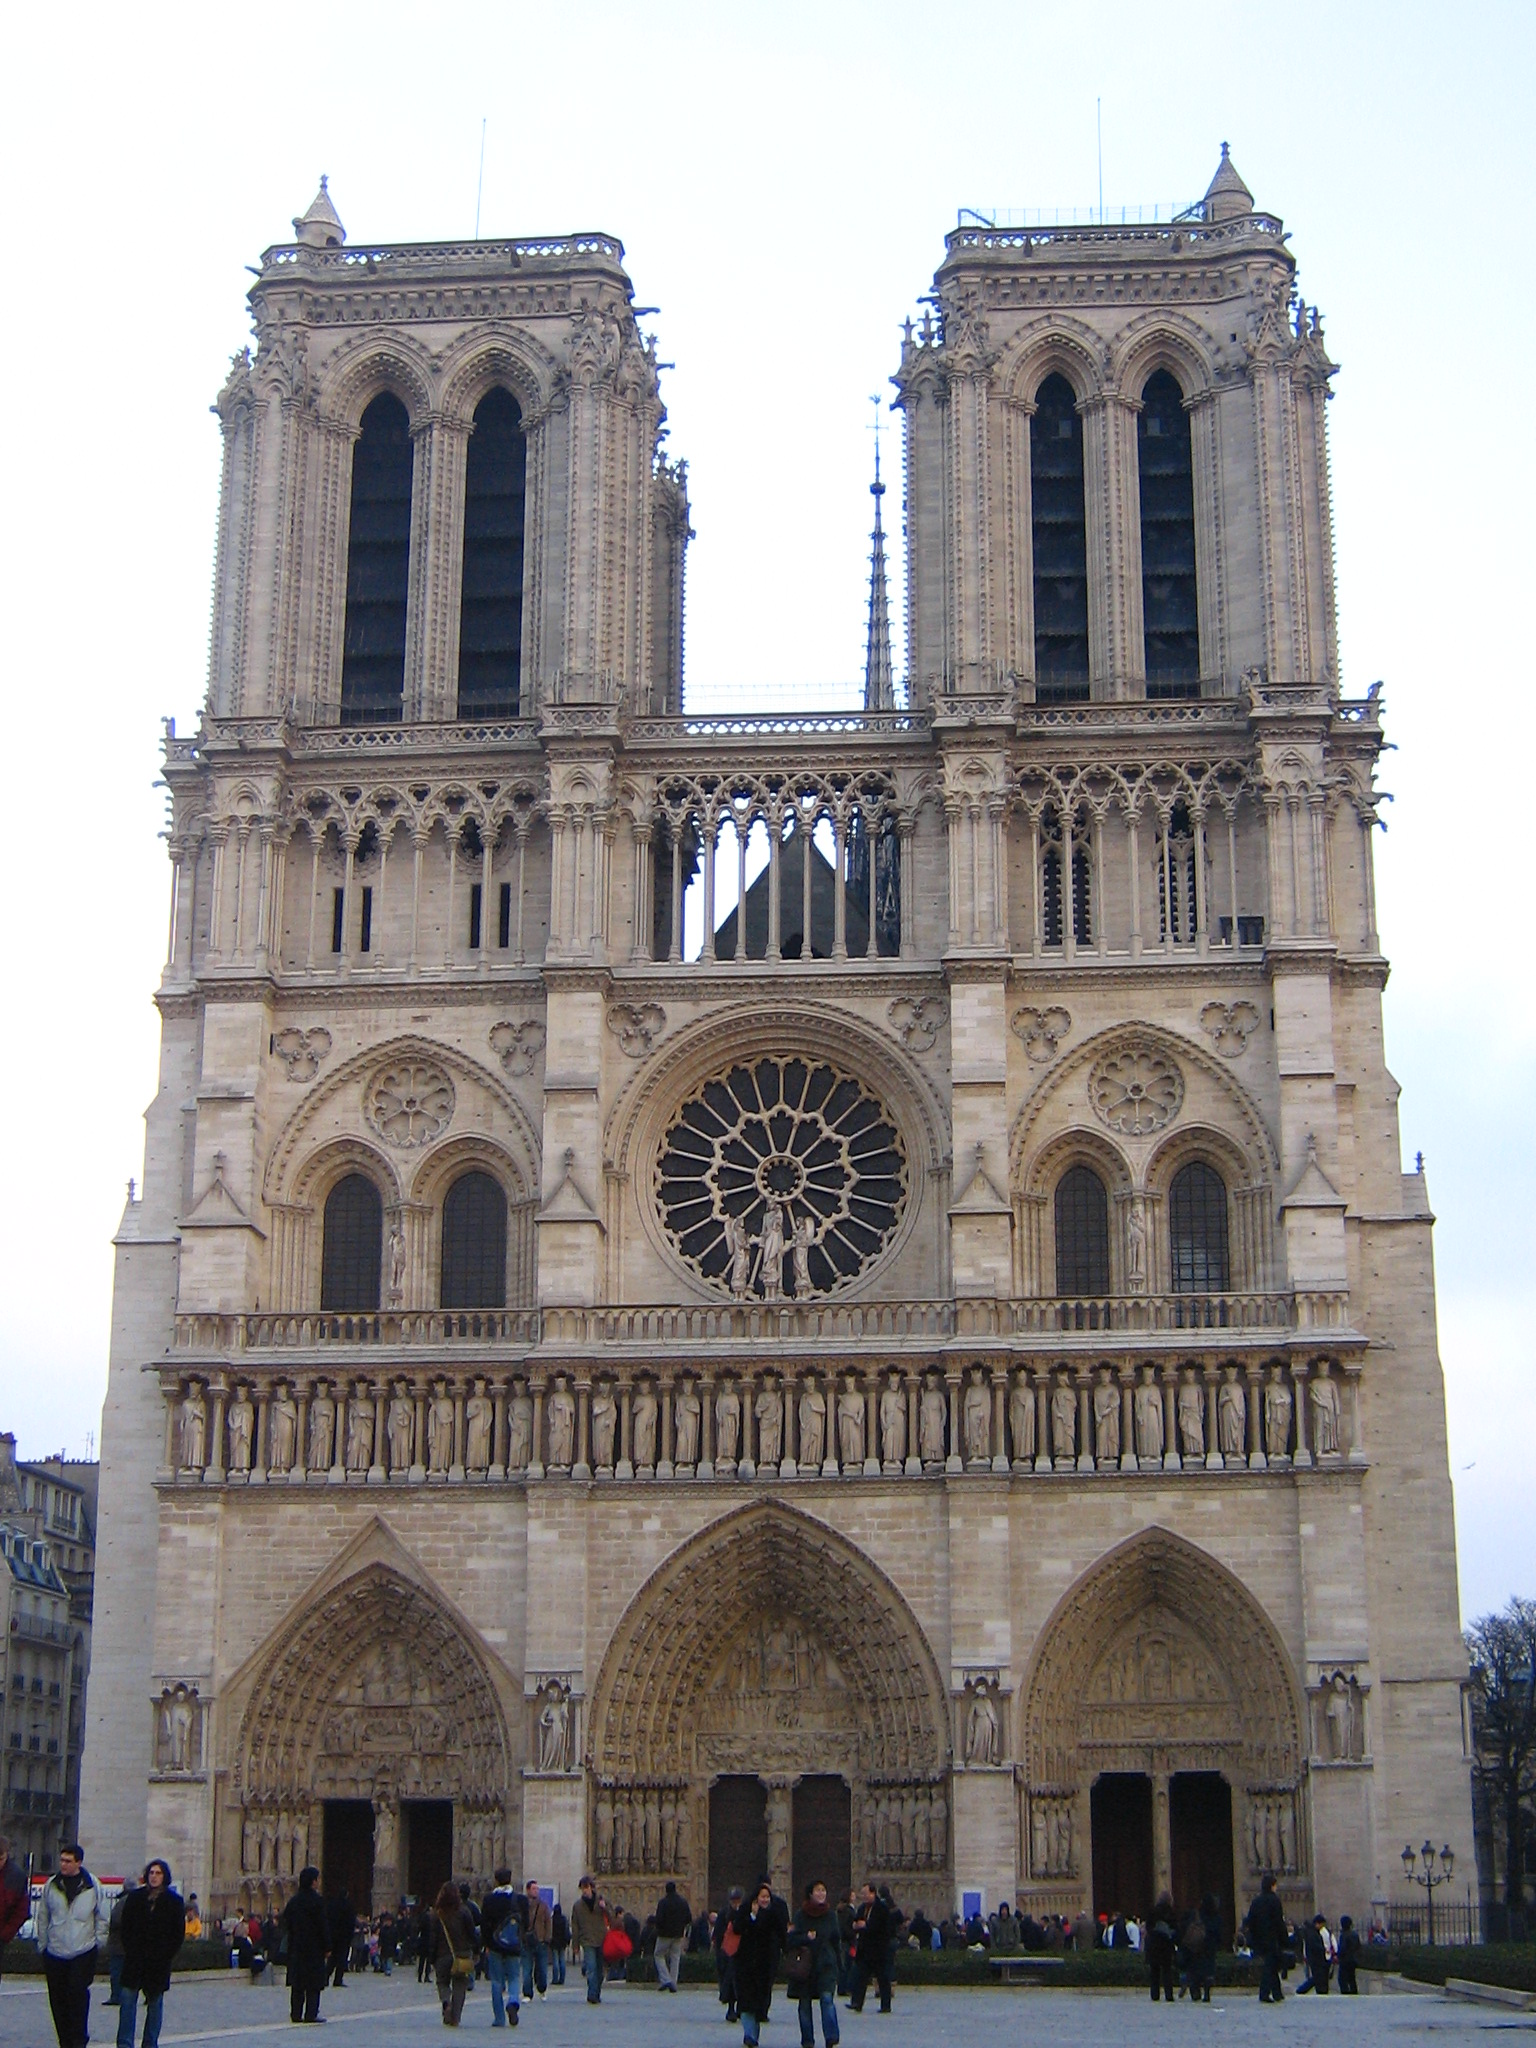
\includegraphics[width=6cm]{images/notre_dame/NotreDame1.jpg}
    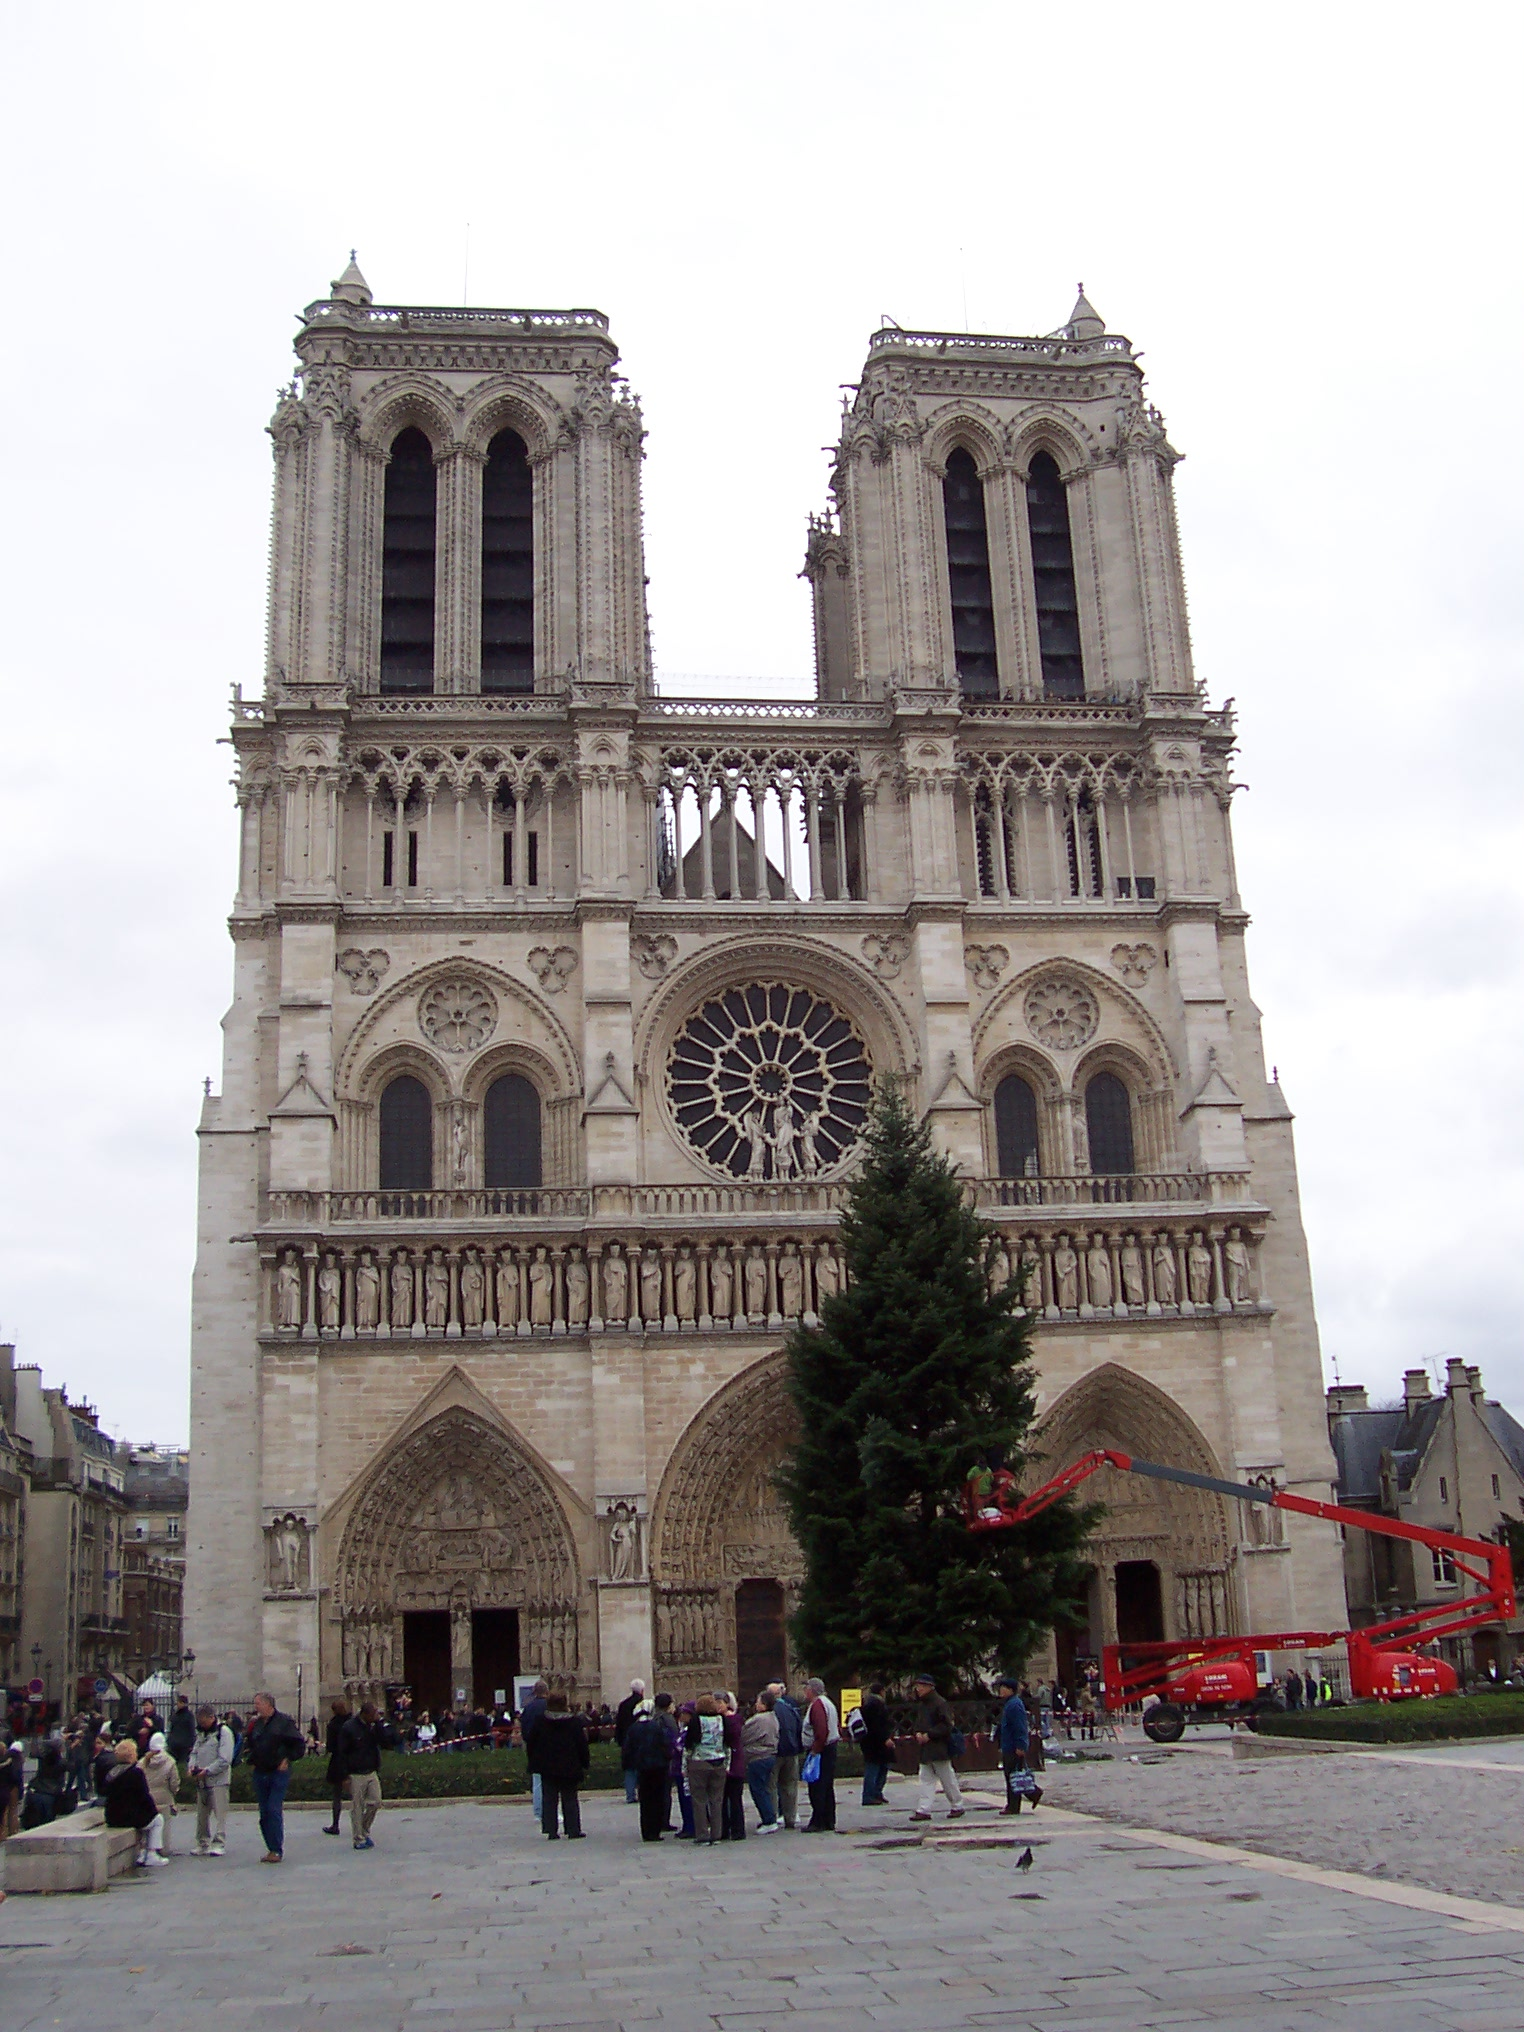
\includegraphics[width=6cm]{images/notre_dame/NotreDame2.jpg}
    \caption{\emph{Left:} Ảnh 1. \emph{Right:} Ảnh 2.}
\end{figure}
Kết quả:
\begin{figure}[H]
    \centering
    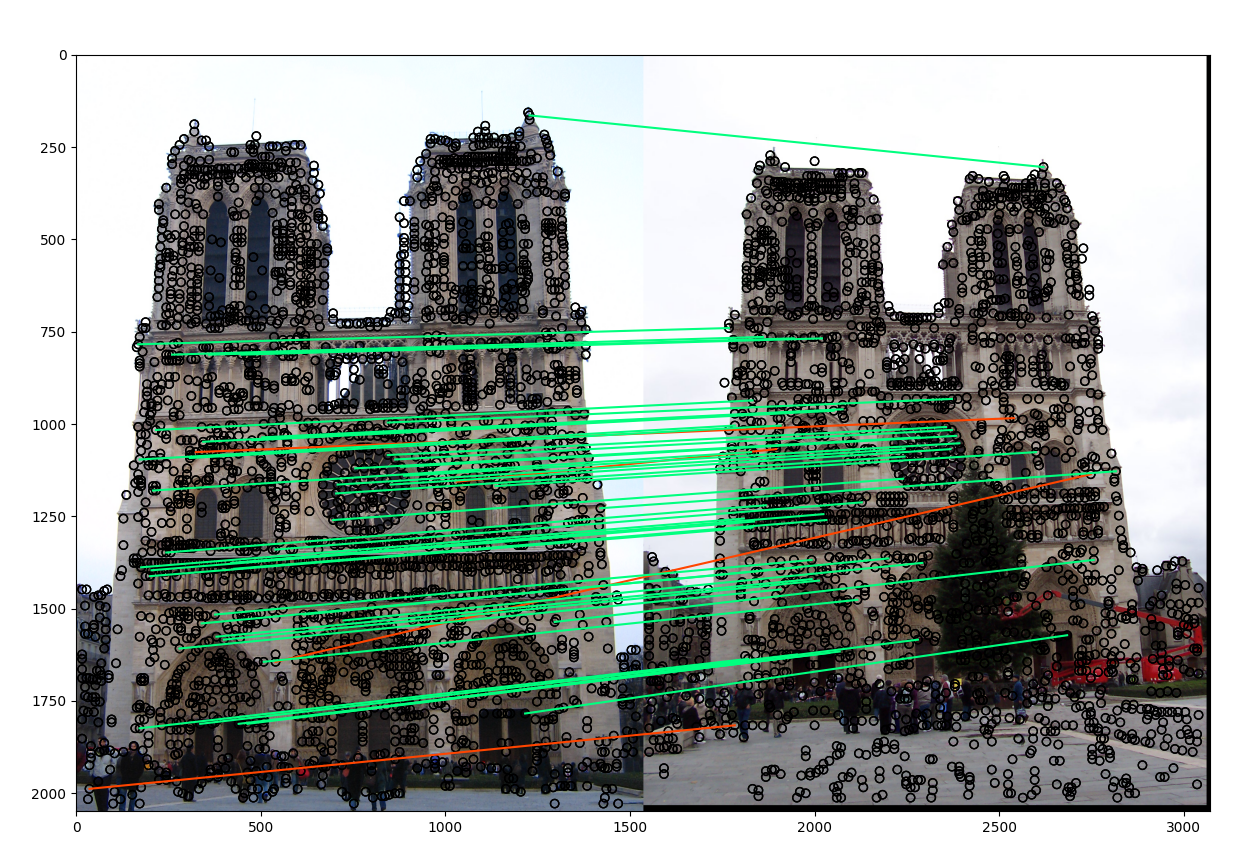
\includegraphics[width=15cm]{images/notre_dame/Figure_1.png}
    \caption{Kết quả sau khi so trùng}
\end{figure}
\begin{verbatim}
Getting interest points...
alpha: 0.06, threshold: 0.01, stride: 2, sigma: 0.1, sigma0: 0.1,
    min_distance: 3
alpha: 0.06, threshold: 0.01, stride: 2, sigma: 0.1, sigma0: 0.1,
    min_distance: 3
Done!
Getting features...
sigma_gradient_image: 0.1, sigma_16x16: 0.4, threshold: 0.2
sigma_gradient_image: 0.1, sigma_16x16: 0.4, threshold: 0.2
Done!
Matching features...
threshold: 0.8
Done!
Matches: 134
Accuracy on 50 most confident: 92%
Accuracy on 100 most confident: 83%
Accuracy on all matches: 82%
\end{verbatim}

\subsection*{MountRushmore}
Ảnh gốc:
\begin{figure}[H]
    \centering
    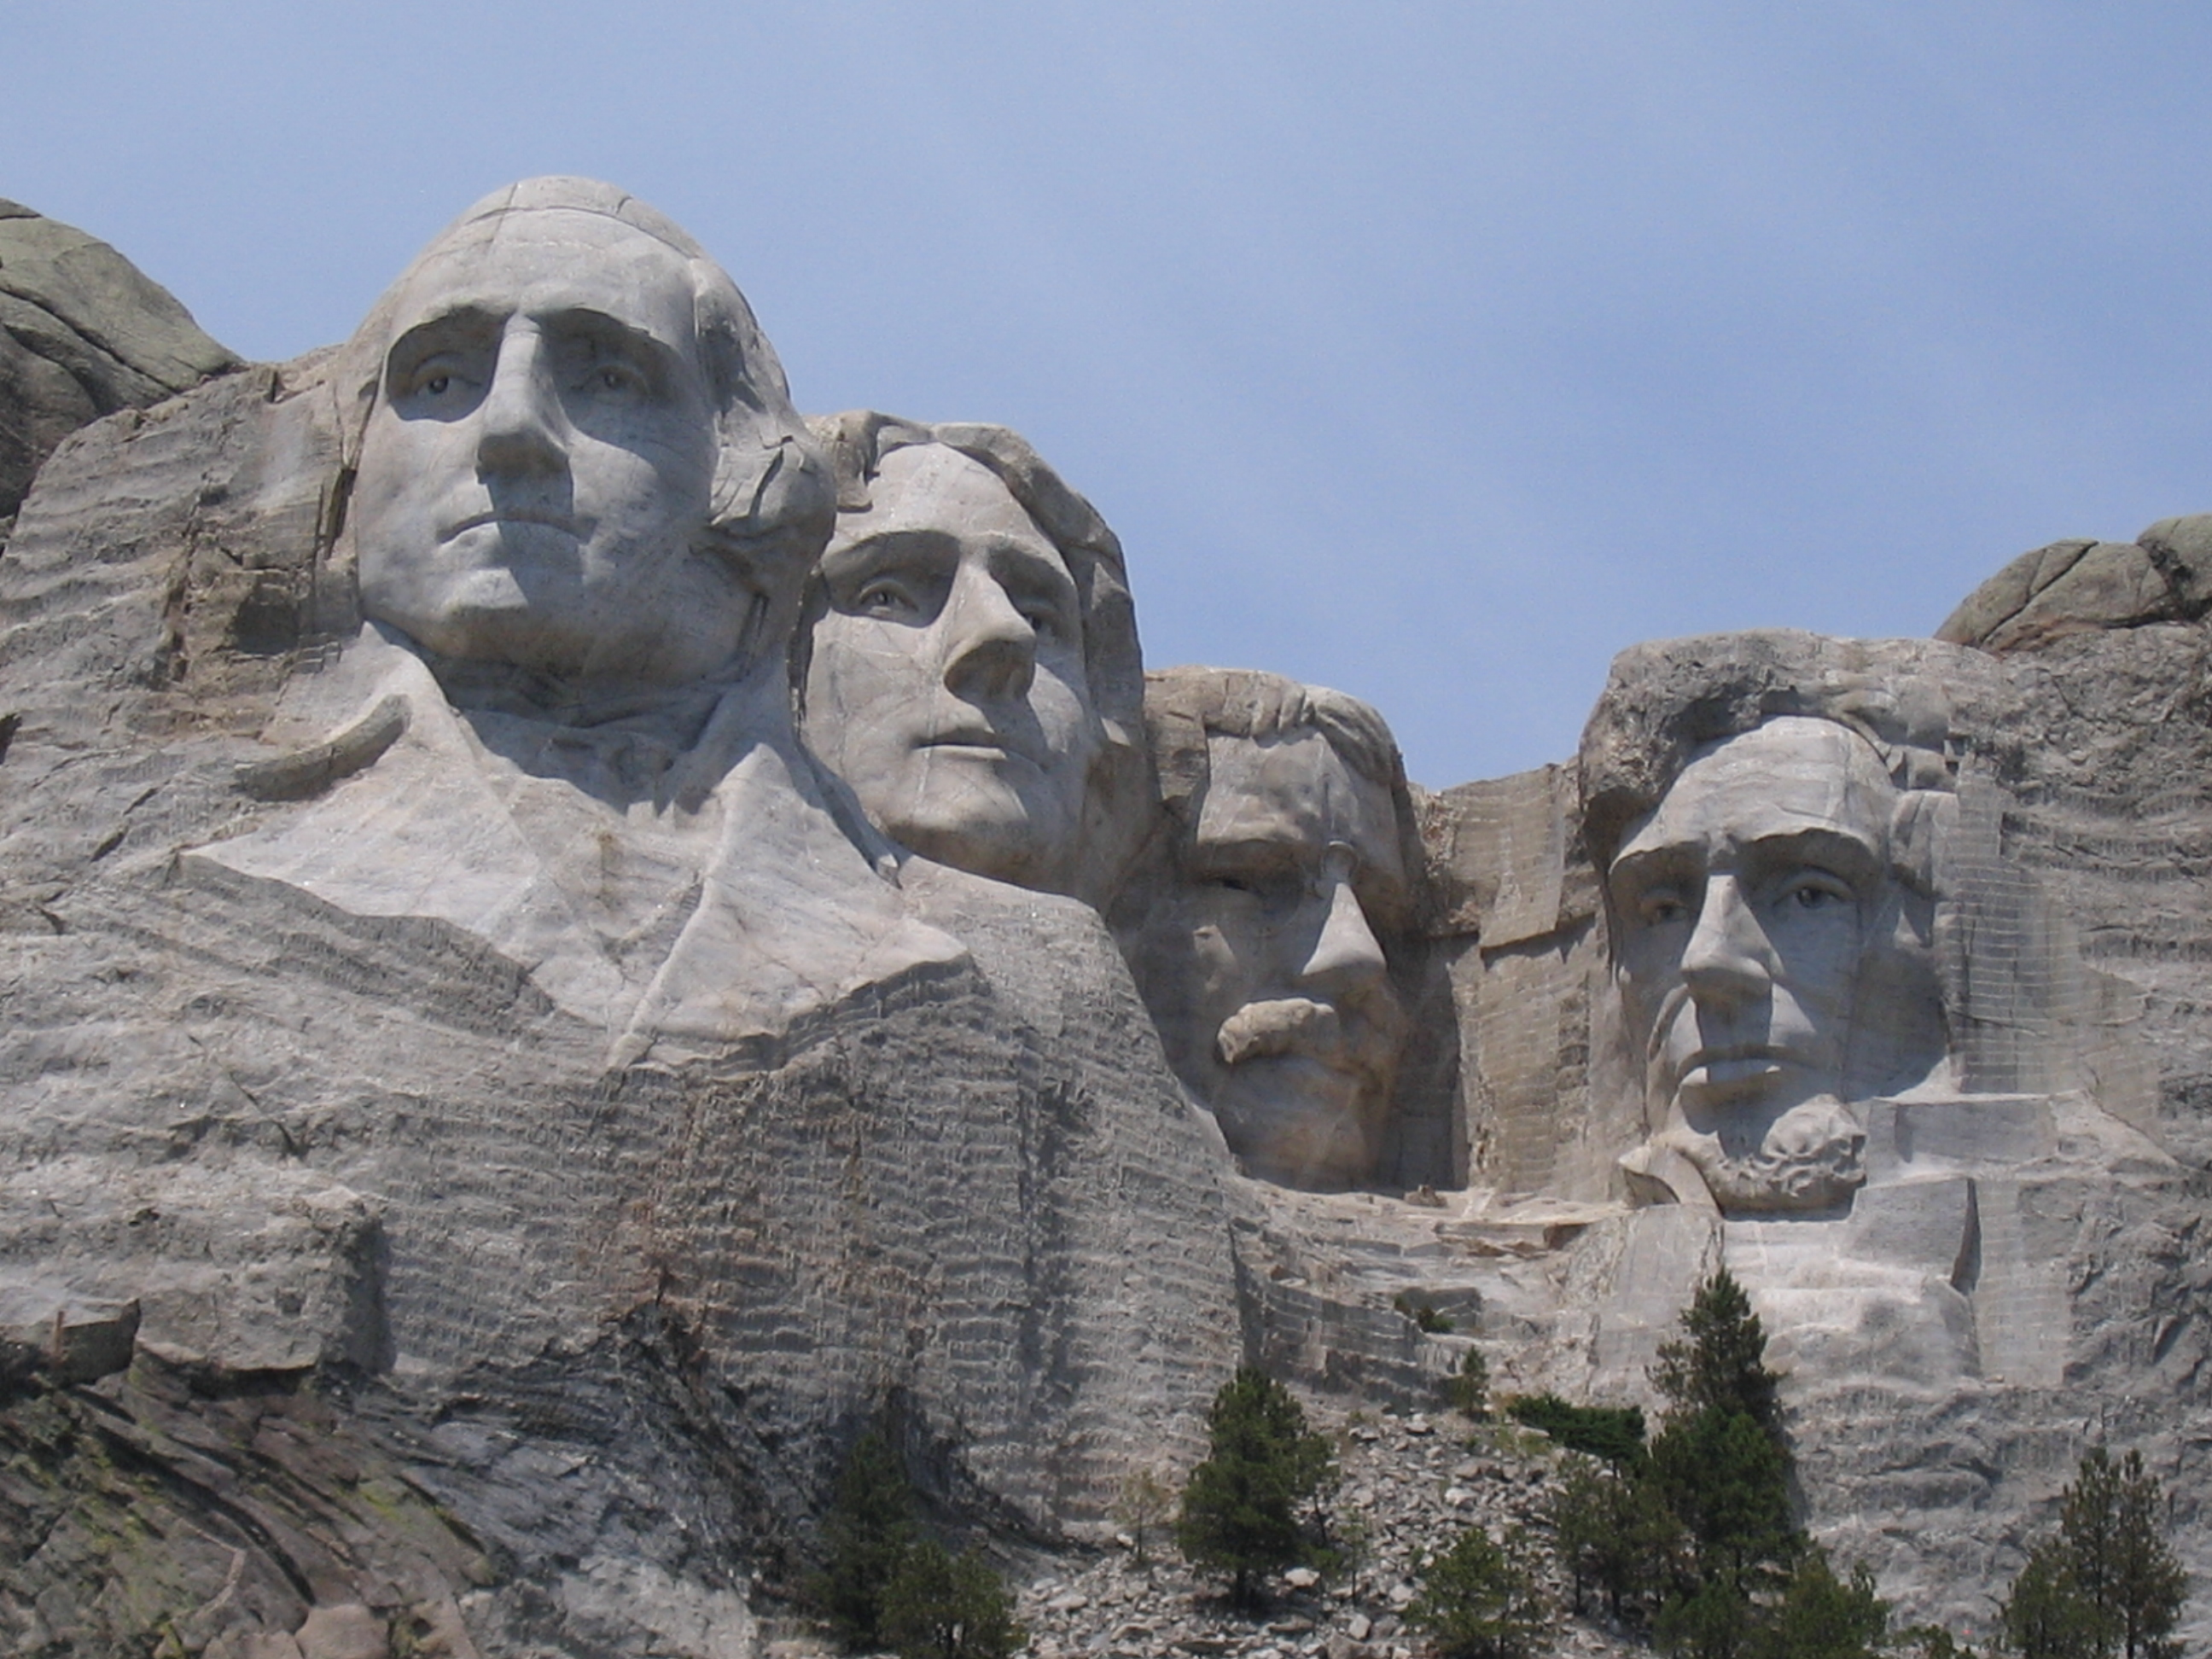
\includegraphics[width=6cm]{images/MountRushmore/Mount_Rushmore1.jpg}
    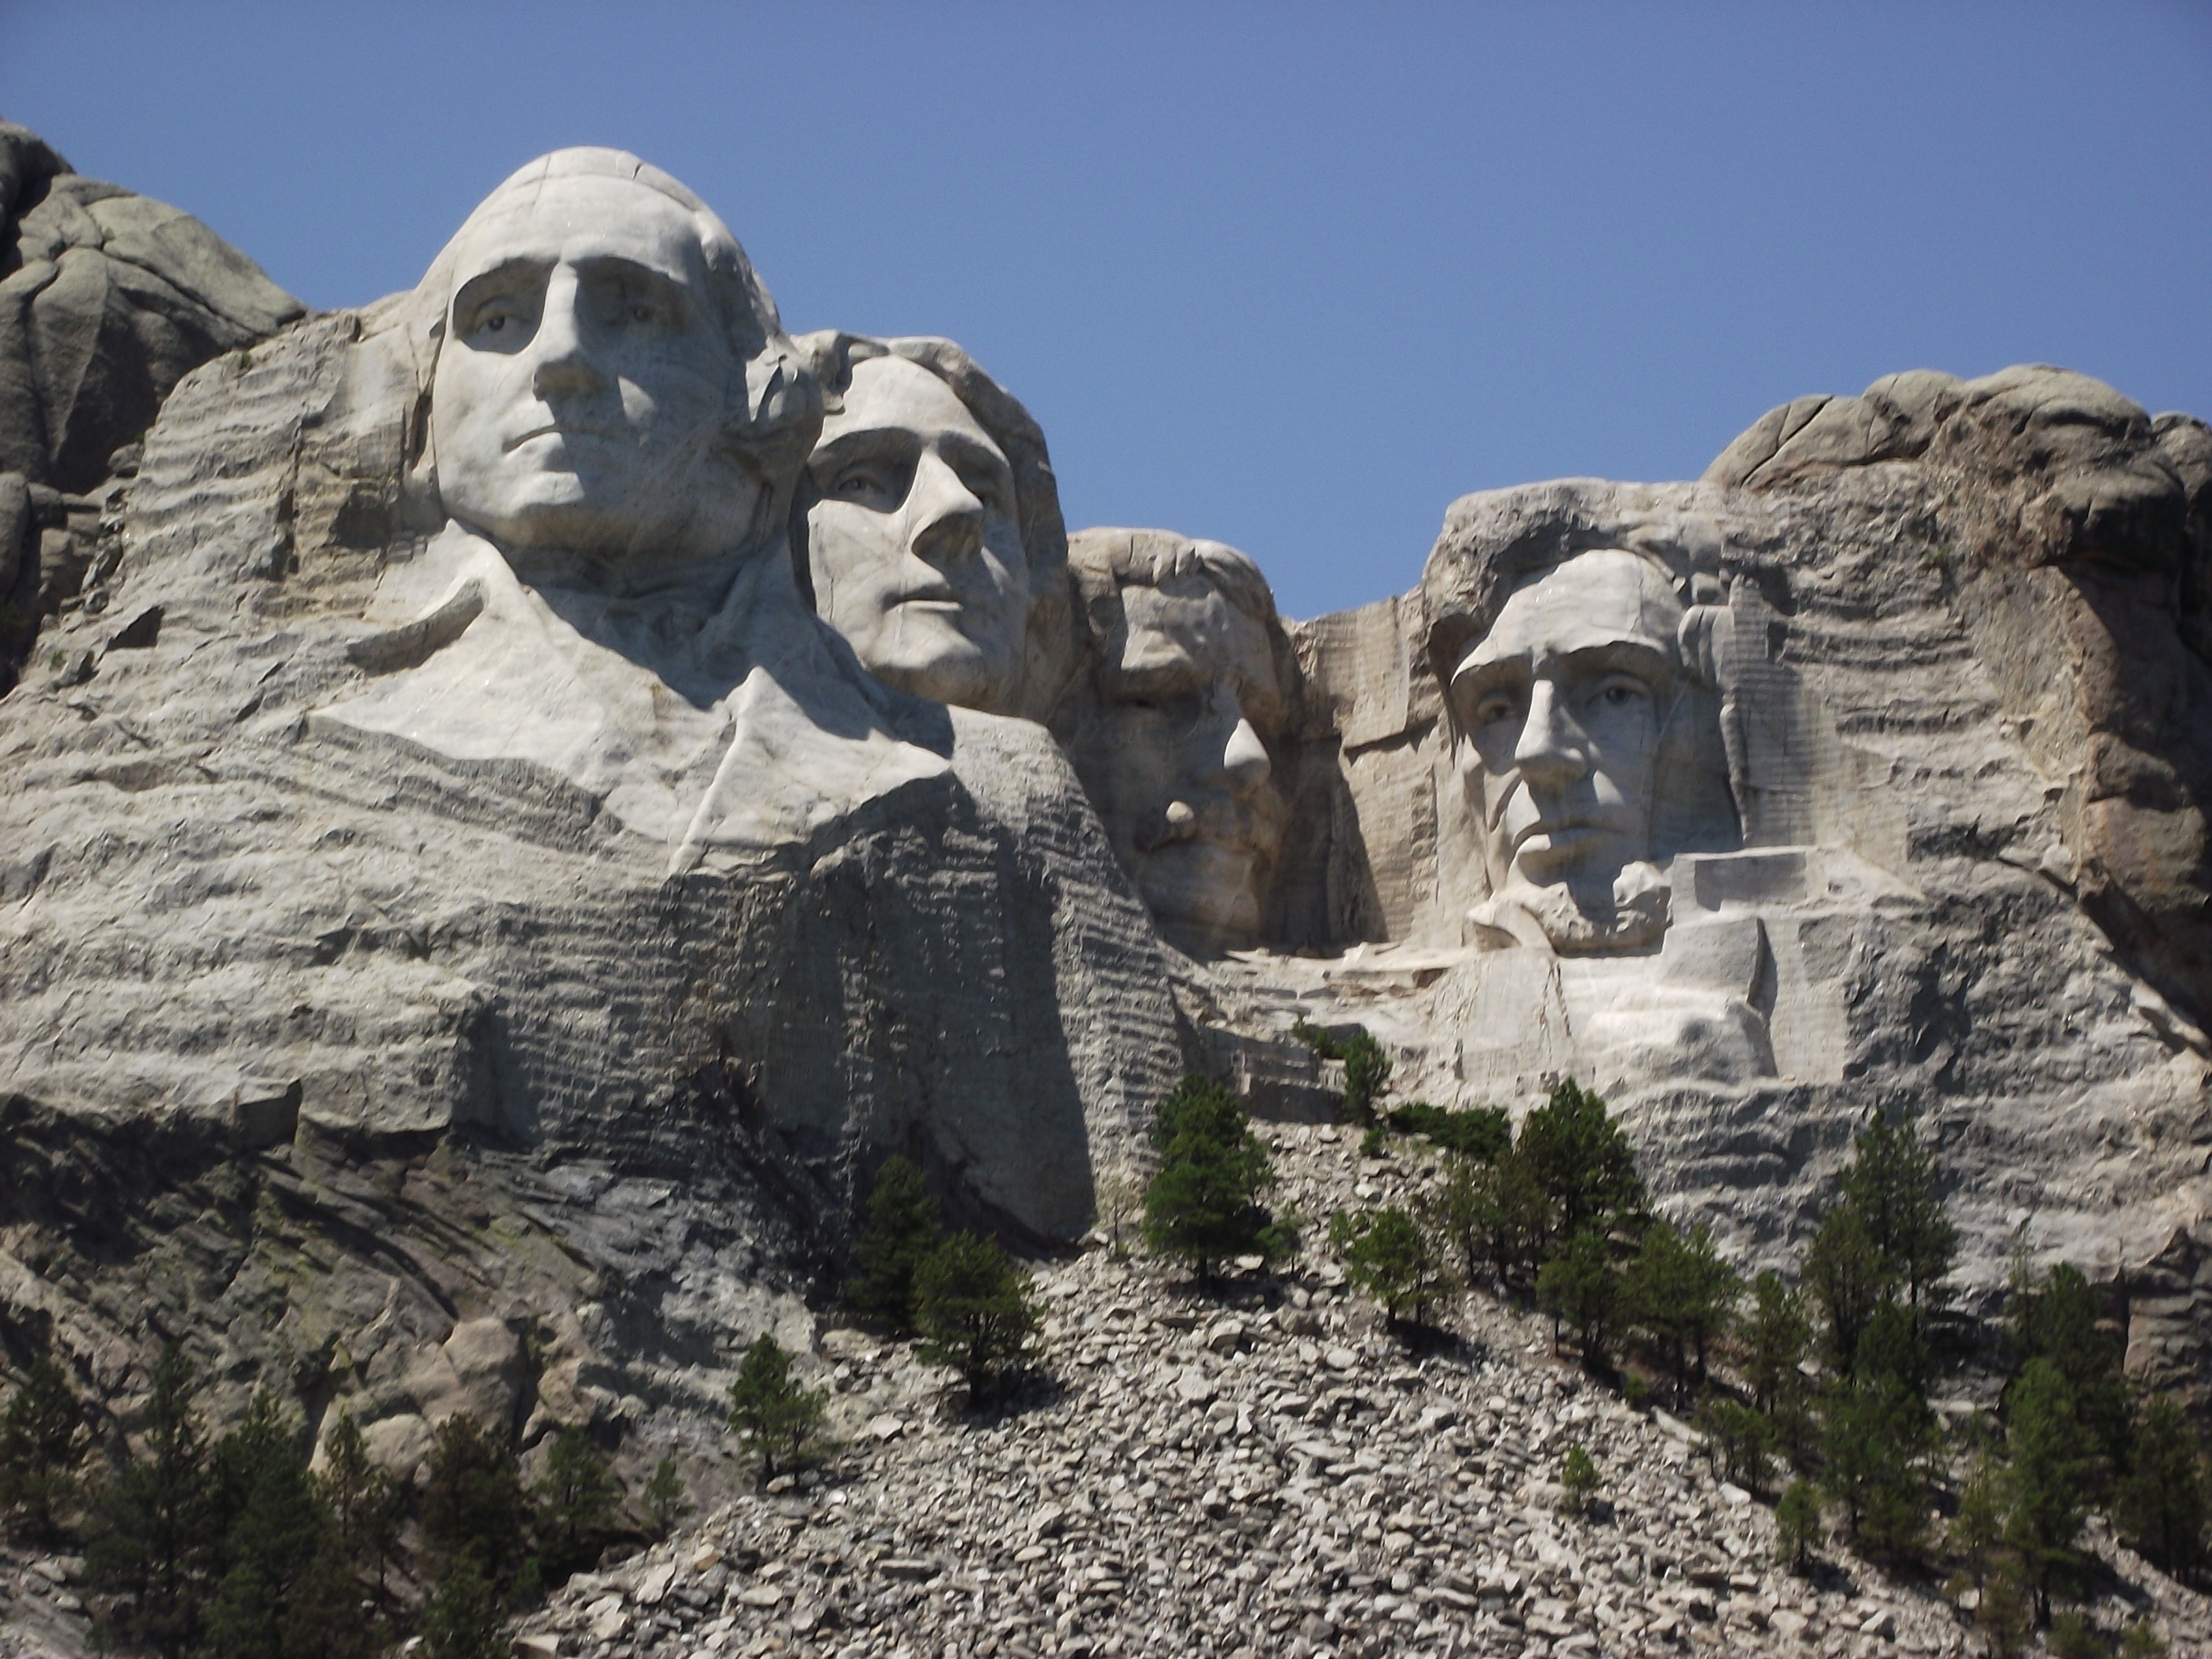
\includegraphics[width=6cm]{images/MountRushmore/Mount_Rushmore2.jpg}
    \caption{\emph{Left:} Ảnh 1. \emph{Right:} Ảnh 2.}
\end{figure}
Kết quả:
\begin{figure}[H]
    \centering
    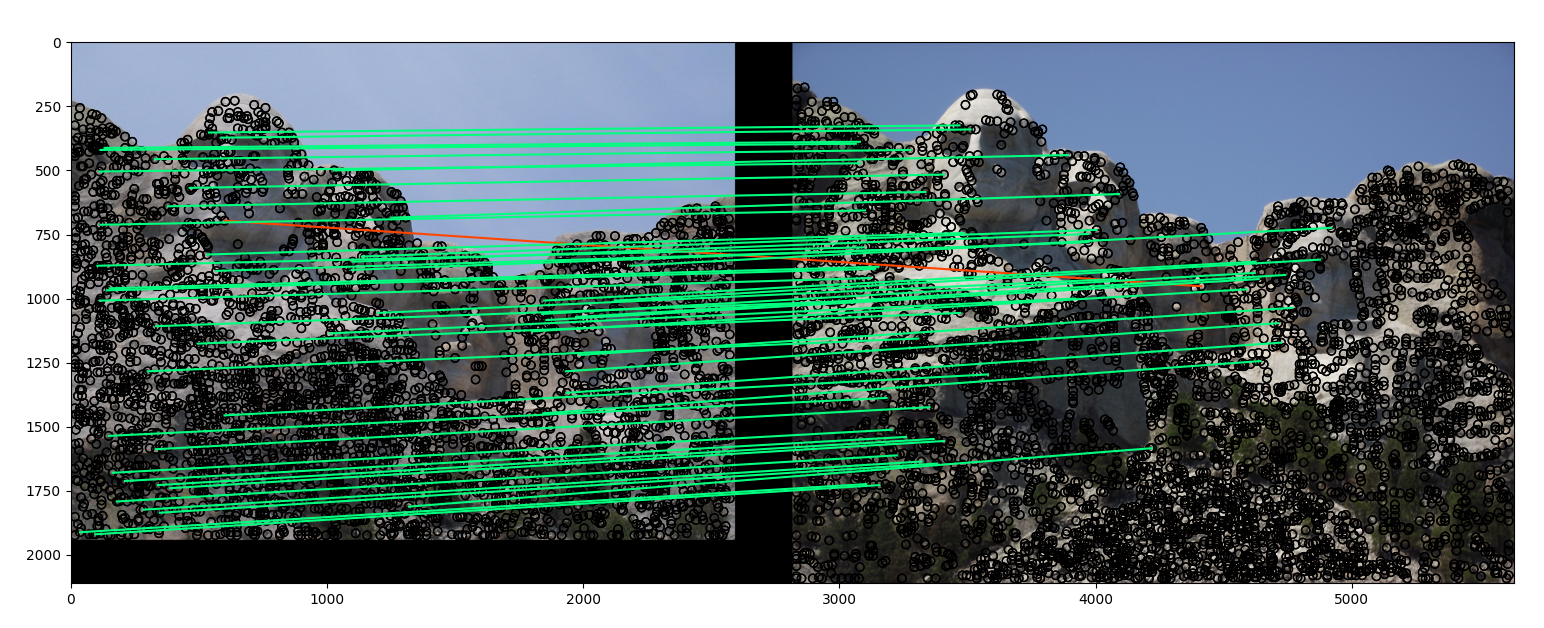
\includegraphics[width=15cm]{images/MountRushmore/Figure_2.png}
    \caption{Kết quả sau khi so trùng}
\end{figure}
\begin{verbatim}
Getting interest points...
alpha: 0.06, threshold: 0.01, stride: 2, sigma: 0.1, sigma0: 0.1,
    min_distance: 3
alpha: 0.06, threshold: 0.01, stride: 2, sigma: 0.1, sigma0: 0.1,
    min_distance: 3
Done!
Getting features...
sigma_gradient_image: 0.1, sigma_16x16: 0.4, threshold: 0.2
sigma_gradient_image: 0.1, sigma_16x16: 0.4, threshold: 0.2
Done!
Matching features...
threshold: 0.8
Done!
Matches: 168
Accuracy on 50 most confident: 98%
Accuracy on 100 most confident: 99%
Accuracy on all matches: 96%
\end{verbatim}

\subsection*{EpiscopalGaudi}
Ảnh gốc:
\begin{figure}[H]
    \centering
    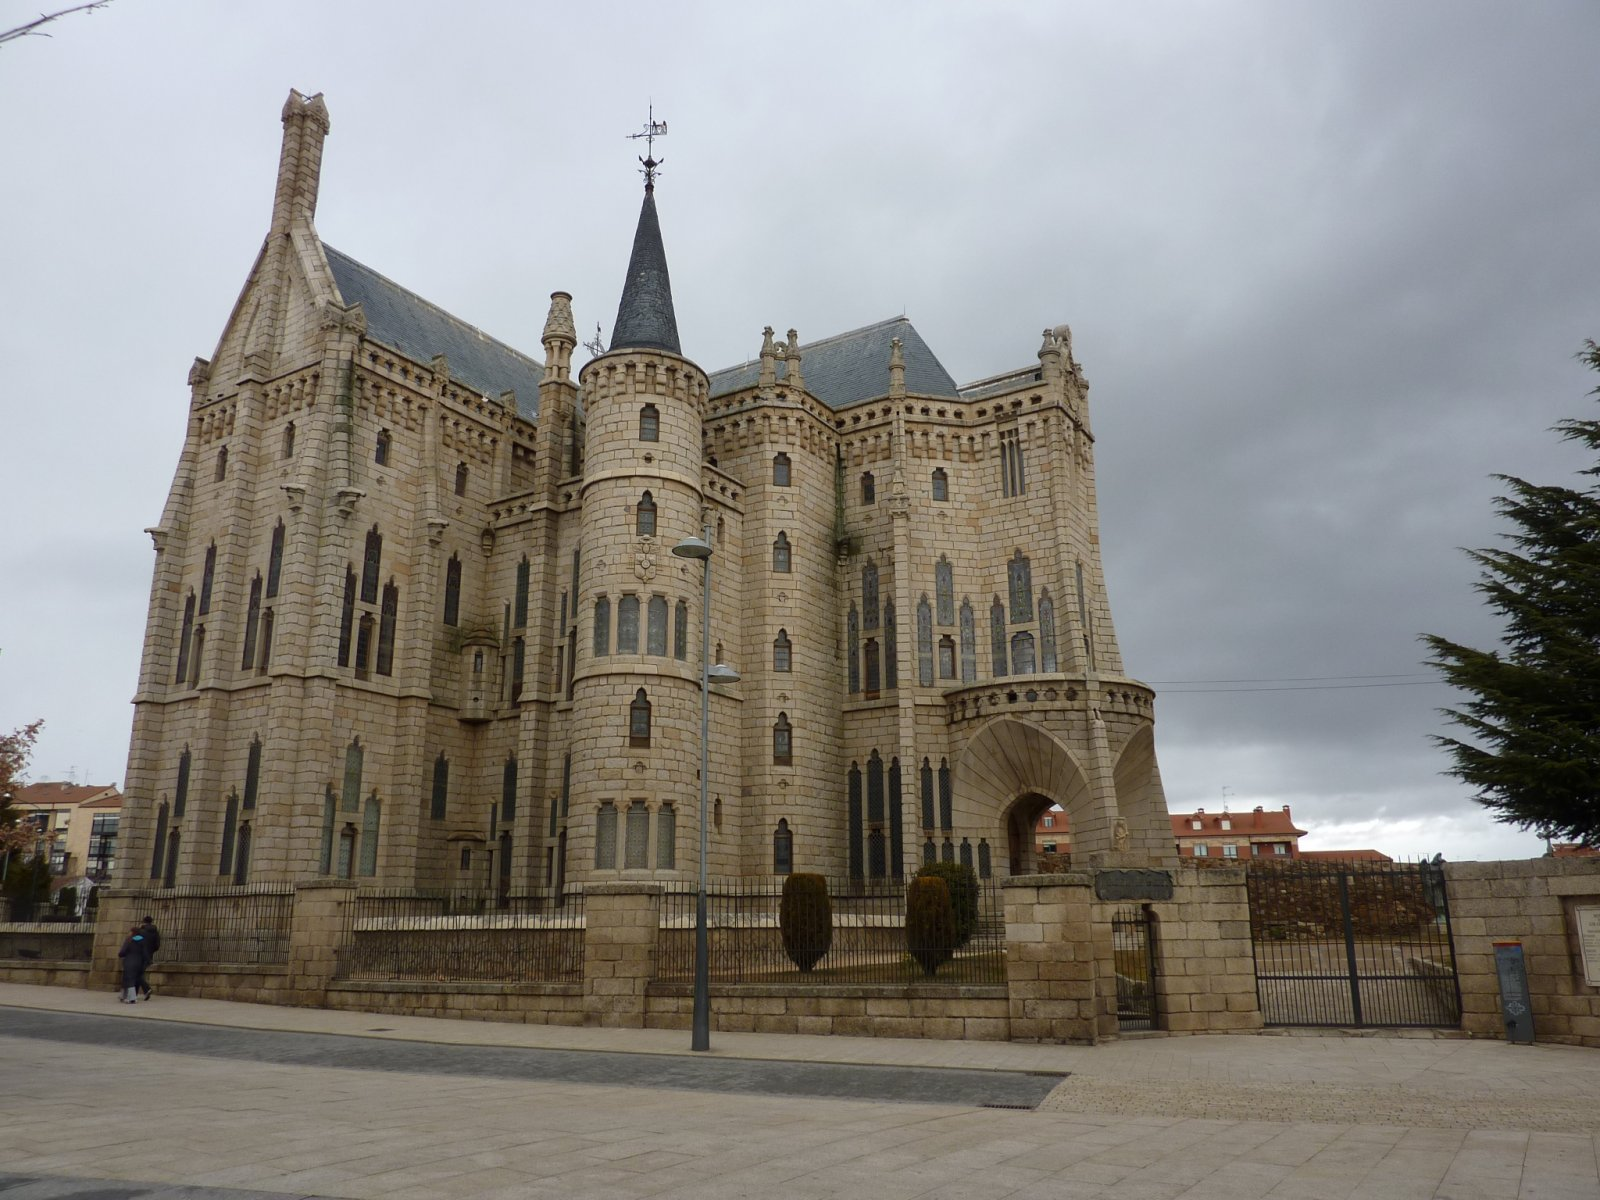
\includegraphics[width=6cm]{images/EpiscopalGaudi/EGaudi_1.jpg}
    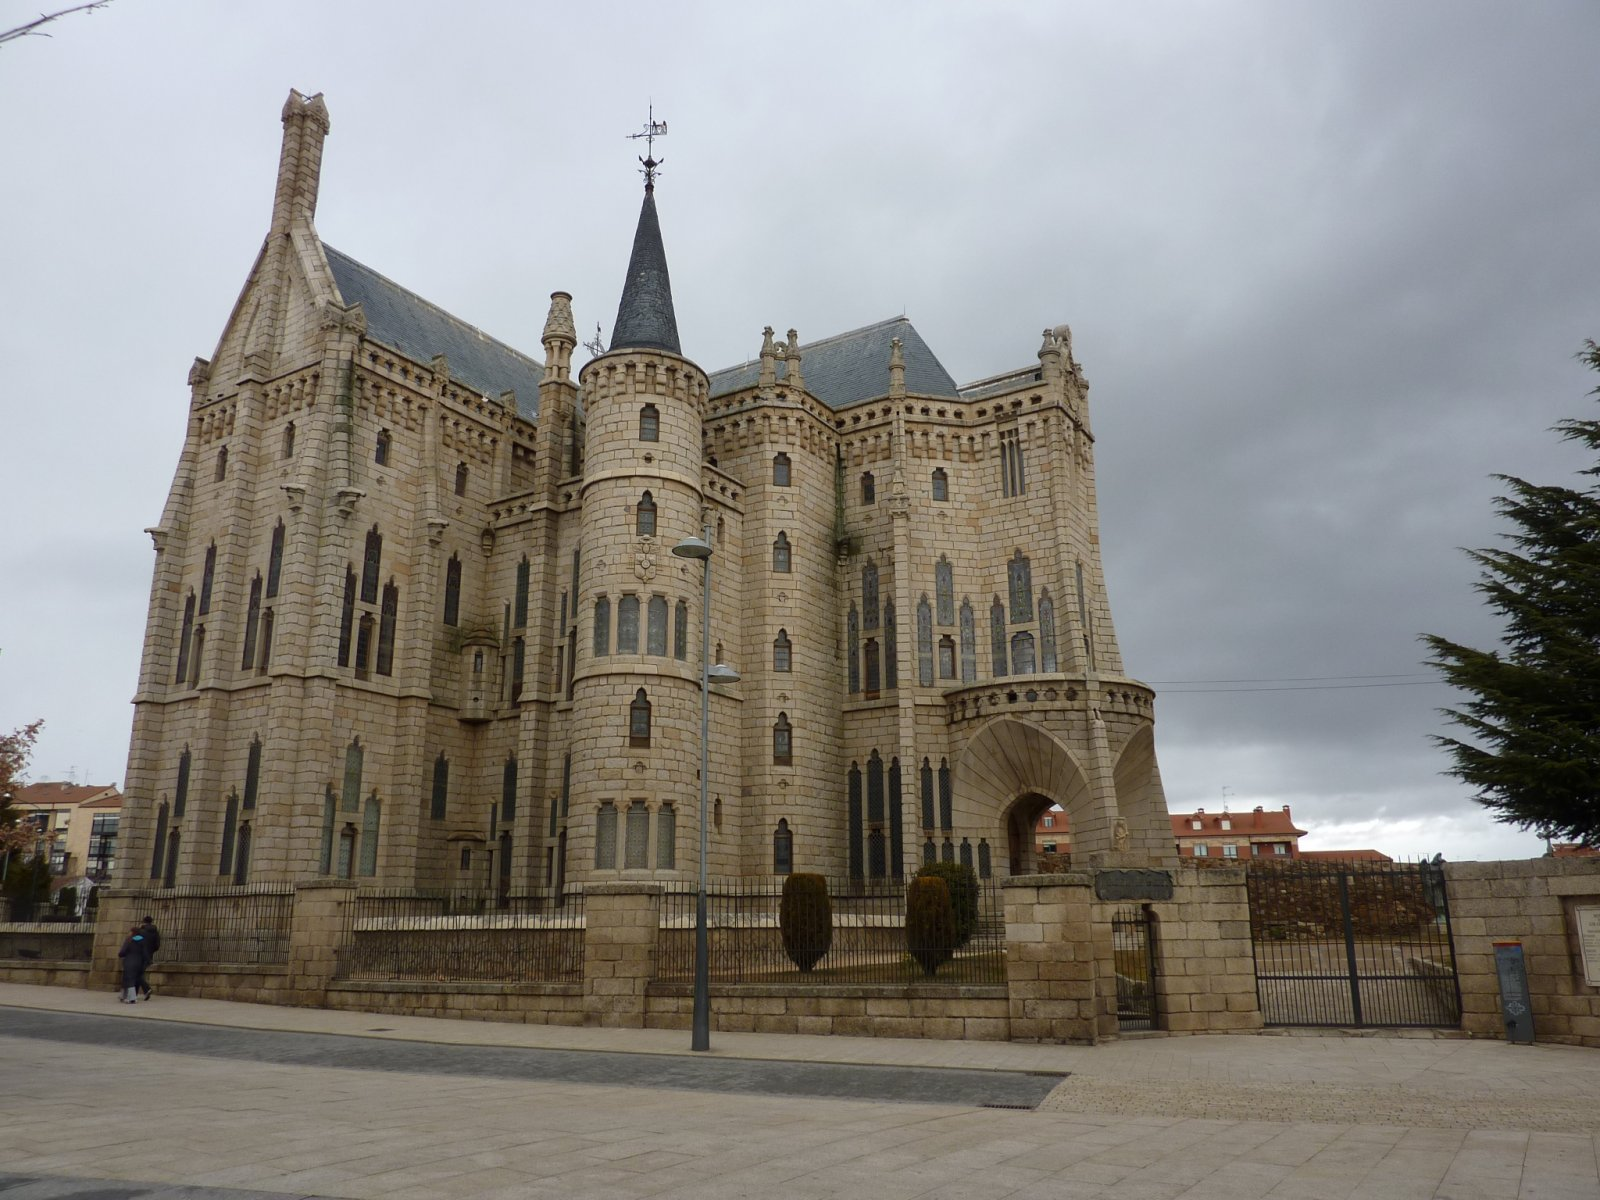
\includegraphics[width=6cm]{images/EpiscopalGaudi/EGaudi_1.jpg}
    \caption{\emph{Left:} Ảnh 1. \emph{Right:} Ảnh 2.}
\end{figure}
Kết quả:
\begin{figure}[H]
    \centering
    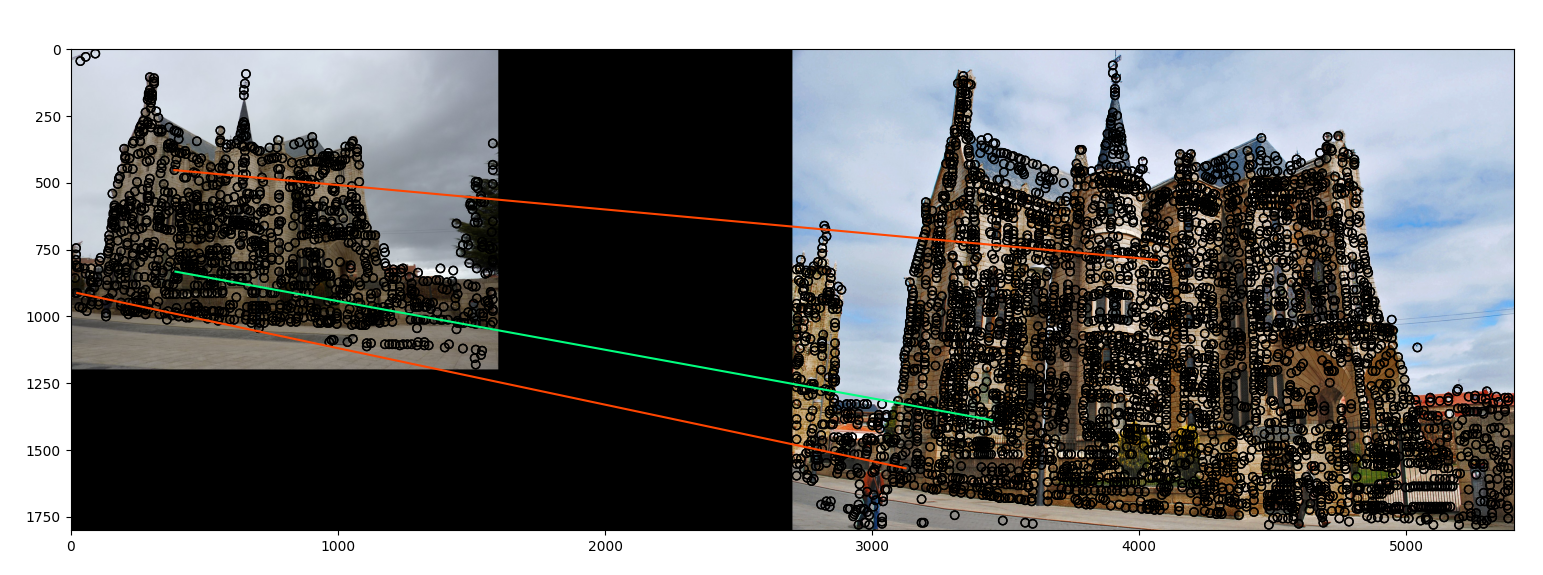
\includegraphics[width=15cm]{images/EpiscopalGaudi/Figure_3.png}
    \caption{Kết quả sau khi so trùng}
\end{figure}
\begin{verbatim}
Getting interest points...
alpha: 0.06, threshold: 0.01, stride: 2, sigma: 0.1, sigma0: 0.1,
    min_distance: 3
alpha: 0.06, threshold: 0.01, stride: 2, sigma: 0.1, sigma0: 0.1,
    min_distance: 3
Done!
Getting features...
sigma_gradient_image: 0.1, sigma_16x16: 0.4, threshold: 0.2
sigma_gradient_image: 0.1, sigma_16x16: 0.4, threshold: 0.2
Done!
Matching features...
threshold: 0.8
Done!
Matches: 3
Accuracy on all matches: 33%
\end{verbatim}

\end{document}
